\documentclass[aspectratio=169,11pt]{beamer}

% ---------------------------------------------------------------- packages --
\usetheme{Madrid}
\usecolortheme{whale}
\usefonttheme{professionalfonts}
\usepackage{lmodern}
\usepackage[T1]{fontenc}
\usepackage{amsmath,amssymb}
\usepackage{graphicx}
\usepackage{booktabs}
\usepackage{array}
\newcolumntype{L}[1]{>{\raggedright\arraybackslash}p{#1}}
\usepackage{xcolor}
\usepackage{siunitx}
\usepackage{tikz}
\usetikzlibrary{positioning,arrows.meta,calc}

\graphicspath{{../figures/}{../final/figures/}}

\setbeamertemplate{navigation symbols}{}
\setbeamertemplate{caption}{\insertcaption}
\setbeamerfont{footnote}{size=\tiny}
\setbeamercolor{block title}{bg=structure!20, fg=black}

\definecolor{good}{RGB}{31,119,180}
\definecolor{bad}{RGB}{214,39,40}
\definecolor{neutral}{RGB}{100,100,100}

\newcommand{\I}{\mathrm{I}}
\newcommand{\HH}{\mathrm{H}}
\newcommand{\Norm}{\mathcal{N}}
\newcommand{\Wb}{\bar{W}}
\newcommand{\smi}{\sigma_{MI}}
\newcommand{\yes}{\textcolor{good}{\textbf{yes}}}
\newcommand{\no}{\textcolor{bad}{\textbf{no}}}

\title[IB theory of deep learning]{On the Information Bottleneck Theory\\of Deep Learning}
\subtitle{A reproduction and critical study}
\author[Information Theory and Inference]{Information Theory and Inference --- course project}
\institute[]{\small after Saxe, Bansal, Dapello, Advani, Kolchinsky, Tracey \& Cox,
           \emph{J.\ Stat.\ Mech.} (2019) 124020}
\date{\today}

\begin{document}

\begin{frame}\titlepage\end{frame}

% ============================================================== background ==
\section{Background: information}

\begin{frame}{Information is surprise}
\begin{columns}[T]
\begin{column}{0.56\textwidth}
An event of probability $p$ carries
\[ \log_2\frac{1}{p} \quad\text{bits of surprise.} \]
Certain event: \SI{0}{bits}. Coin flip: \SI{1}{bit}.
One particular pattern out of 4096: \SI{12}{bits}.
\medskip

\textbf{Entropy} is average surprise:
\[ \HH(X) = -\sum_x p(x)\log_2 p(x) \]
\smallskip
Equivalently: the average number of yes/no questions needed to pin $X$ down --- the
length of the best possible code.
\end{column}
\begin{column}{0.42\textwidth}
\begin{block}{Everything in this talk, in these units}
\small
\begin{tabular}{@{}lr@{}}
\toprule
fair coin & \SI{1.000}{bit}\\
our labels ($p = 0.517$) & \SI{0.999}{bits}\\
12 uniform bits & \SI{12.000}{bits}\\
a constant & \SI{0}{bits}\\
\bottomrule
\end{tabular}
\end{block}
\medskip
\footnotesize
A bit is a unit of \emph{uncertainty}. Everything that follows is bookkeeping on
uncertainty --- and the whole argument will turn on \emph{whose} uncertainty we
are counting.
\end{column}
\end{columns}
\end{frame}

\begin{frame}{Mutual information: what one variable tells you about another}
\begin{columns}[T]
\begin{column}{0.54\textwidth}
\[ \I(X;T) \;=\; \underbrace{\HH(X)}_{\text{before}} - \underbrace{\HH(X\mid T)}_{\text{after}} \]
\emph{The uncertainty about $X$ that knowing $T$ removes.}\\[4pt]
{\small Equivalently \ $\HH(T)-\HH(T\mid X)$ \ or \ $\HH(X)+\HH(T)-\HH(X,T)$ ---
all three are used later.}
\medskip
\begin{block}{\small Three properties that will matter}
\footnotesize
\begin{enumerate}
  \item symmetric, $\ge 0$, and $=0$ exactly when independent;
  \item \textbf{invariant} under any invertible transform of $X$ or $T$ ---
        \emph{the} reason to reach for it;
  \item \textbf{DPI}: if $X\to A\to B$ then $\I(X;A)\ge\I(X;B)$ --- processing cannot
        create information.
\end{enumerate}
\end{block}
\end{column}
\begin{column}{0.44\textwidth}
\centering
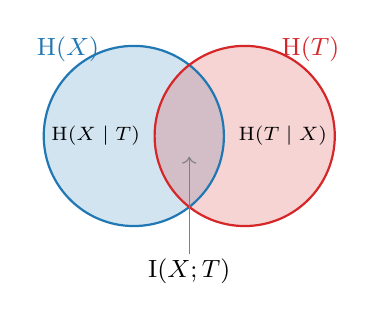
\begin{tikzpicture}[scale=0.88]
  \fill[good, opacity=0.20] (0,0) circle (1.3);
  \fill[bad,  opacity=0.20] (1.6,0) circle (1.3);
  \draw[good, thick] (0,0) circle (1.3);
  \draw[bad,  thick] (1.6,0) circle (1.3);
  \node[good, font=\small] at (-0.95,1.25) {$\HH(X)$};
  \node[bad,  font=\small] at ( 2.55,1.25) {$\HH(T)$};
  \node[font=\scriptsize] at (-0.55,0) {$\HH(X\mid T)$};
  \node[font=\scriptsize] at ( 2.15,0) {$\HH(T\mid X)$};
  \node[font=\small\bfseries] at (0.8,-1.95) {$\I(X;T)$};
  \draw[->, gray] (0.8,-1.7) -- (0.8,-0.3);
\end{tikzpicture}
\\[4pt]
\footnotesize The overlap. Property 2 says it does not care what \emph{units} you
measure $X$ and $T$ in --- keep that in mind for slide \ref{fig:rescale}.
\end{column}
\end{columns}
\end{frame}

\begin{frame}{Computing it, case 1: discrete variables --- easy}
\begin{columns}[T]
\begin{column}{0.52\textwidth}
Count the joint table, normalise, sum:
\[ \hat{\I}(X;T)=\sum_{x,t}\hat p(x,t)\,\log_2\frac{\hat p(x,t)}{\hat p(x)\,\hat p(t)} \]
\medskip
\footnotesize
\begin{tabular}{@{}c|cc|c@{}}
\toprule
$p(x,t)$ & $t{=}0$ & $t{=}1$ & \\
\midrule
$x{=}0$ & 0.4 & 0.1 & 0.5\\
$x{=}1$ & 0.1 & 0.4 & 0.5\\
\midrule
        & 0.5 & 0.5 & \\
\bottomrule
\end{tabular}
\quad$\Rightarrow\ \I = \SI{0.278}{bits}$
\normalsize
\medskip

Marginals are uniform (\SI{1}{bit} each), but the pair agrees \SI{80}{\percent} of the
time --- so $T$ answers a bit over a quarter of the question ``what is $X$?''.
\end{column}
\begin{column}{0.46\textwidth}
\begin{alertblock}{The catch: plug-in bias}
\footnotesize
With $P$ samples and many distinct values, $\hat\I$ \textbf{over}estimates.\\[3pt]
In the limit where every sample is unique, $T$ identifies the sample, hence its
label, and
\[ \hat\I(T;Y) = \HH(Y) \]
\emph{no matter what the truth is}. Resolution and sample size are not free
parameters.
\end{alertblock}
\footnotesize
It bites in our own data: 8 random units at 30 bins ``know'' \SI{1.0}{bit} about a
label they are independent of.
\end{column}
\end{columns}
\end{frame}

\begin{frame}{Computing it, case 2: continuous variables --- treacherous}
Replace the sum by an integral: \ $h(X)=-\int p(x)\log_2 p(x)\,dx$ \ (\emph{differential} entropy).
\medskip
\begin{columns}[T]
\begin{column}{0.48\textwidth}
\begin{alertblock}{Three things change}
\footnotesize
\begin{enumerate}
  \item it can be \textbf{negative} (a narrow Gaussian);
  \item it is \textbf{not invariant}: $h(cX)=h(X)+\log_2|c|$ --- it depends on the
        units you chose;
  \item it is not a limit of the discrete entropy --- that diverges.
\end{enumerate}
\end{alertblock}
\footnotesize
$\I$ survives all three: the two $\log_2 c$ terms cancel, so mutual information
\emph{is} still invariant. That is why people trust it.
\end{column}
\begin{column}{0.50\textwidth}
\begin{block}{But we never have $p$ --- only samples}
\footnotesize
Three ways out, and every one is an \textbf{added assumption}:
\begin{itemize}
  \item \textbf{discretise} $\Rightarrow$ pick a resolution
  \item \textbf{smooth} (KDE) $\Rightarrow$ pick a bandwidth / noise level
  \item \textbf{nearest neighbours} $\Rightarrow$ assume a density exists at all
\end{itemize}
\end{block}
\medskip
\centering
\footnotesize\textcolor{bad}{Hold that thought.}\\ It is the whole talk.
\end{column}
\end{columns}
\end{frame}

% ============================================================== motivation ==
\section{The claim}

\begin{frame}{The information bottleneck (Tishby, Pereira \& Bialek 1999)}
\begin{columns}[T]
\begin{column}{0.54\textwidth}
Find a representation $T$ of the input $X$ that is
\begin{itemize}
  \item as \textbf{informative} about the label $Y$ as possible,
  \item as \textbf{compressed} about $X$ as possible.
\end{itemize}
\[ \min_{p(t\mid x)}\ \ \I(X;T) \;-\; \beta\,\I(T;Y) \]
\begin{itemize}\small
  \item $\beta \to 0$: keep nothing
  \item $\beta \to \infty$: keep everything ($T = X$)
  \item sweeping $\beta$ traces the \textbf{IB curve} --- the best $\I(T;Y)$
        achievable at each $\I(X;T)$
\end{itemize}
\medskip
\footnotesize
It is rate--distortion theory with $\I(T;Y)$ as the fidelity measure: a
\emph{soft} version of a minimal sufficient statistic.
\end{column}
\begin{column}{0.44\textwidth}
\centering
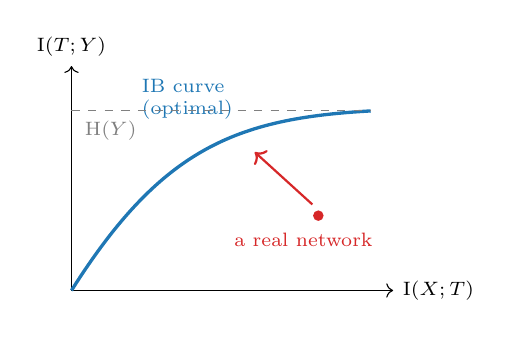
\begin{tikzpicture}[scale=0.95]
  \draw[->] (0,0)--(4.3,0) node[right, font=\scriptsize] {$\I(X;T)$};
  \draw[->] (0,0)--(0,3.0) node[above, font=\scriptsize] {$\I(T;Y)$};
  \draw[good, very thick] (0,0) .. controls (1.2,1.9) and (2.2,2.3) .. (4.0,2.4);
  \node[good, font=\scriptsize, align=left] at (1.55,2.55) {IB curve\\(optimal)};
  \draw[dashed, gray] (0,2.4)--(4.0,2.4);
  \node[gray, font=\scriptsize, below right] at (0.05,2.4) {$\HH(Y)$};
  \fill[bad] (3.3,1.0) circle (2pt);
  \node[bad, font=\scriptsize, below] at (3.1,0.9) {a real network};
  \draw[->, bad, thick] (3.22,1.15) -- (2.45,1.85);
\end{tikzpicture}\\[4pt]
\footnotesize Everything below the curve is achievable; the curve itself is the
frontier. ``Learning well'' is supposed to mean \emph{moving towards it}.
\end{column}
\end{columns}
\end{frame}

\begin{frame}{From a principle to a theory of deep learning (Tishby \& Zaslavsky 2015)}
\small
A feed-forward network is \emph{already} a Markov chain:
\[ Y \to X \to T_1 \to T_2 \to \cdots \to T_L \to \hat{Y} \]
so the DPI applies to it directly, and gives for free
\[ \I(X;T_1) \ge \I(X;T_2) \ge \cdots \ge \I(X;T_L),
\qquad \I(T_1;Y) \ge \cdots \ge \I(T_L;Y). \]
\smallskip
\begin{columns}[T]
\begin{column}{0.49\textwidth}
\begin{block}{The proposal}
Each layer is a successively compressed representation. Training \emph{should} drive
the layers towards the IB curve --- and the depth of the network is what lets it get
there in feasible steps.
\end{block}
\end{column}
\begin{column}{0.49\textwidth}
\begin{block}{Why anyone should care}
\begin{itemize}\small
  \item a single, \textbf{architecture-agnostic} currency: bits
  \item an \emph{optimality} target, not just a loss curve
  \item $\I(X;T)$ as a complexity measure $\Rightarrow$ a route to a
        generalisation bound
\end{itemize}
\end{block}
\end{column}
\end{columns}
\medskip
\centering\small
An attractive programme. The question is whether the quantity plotted is the one in the theory.
\end{frame}

\begin{frame}{The information plane}
\begin{columns}[T]
\begin{column}{0.56\textwidth}
Treat each hidden layer $T$ as a summary statistic of the input:
\[ Y \to X \to T_1 \to T_2 \to \cdots \to \hat{Y} \]
Plot, for each layer and each epoch,
\[ \I(T;Y) \ \text{ against } \ \I(X;T). \]
\medskip
\textbf{Why it is appealing}
\begin{itemize}
  \item architecture-agnostic --- a common currency
  \item the IB principle gives an optimal frontier
    \[ \mathcal{L} = \I(X;T) - \beta\,\I(T;Y) \]
\end{itemize}
\end{column}
\begin{column}{0.42\textwidth}
\begin{block}{Reading the plot}
\begin{itemize}
  \item[$\rightarrow$] right = \emph{fitting} (learns about input)
  \item[$\uparrow$] up = \emph{fitting} (learns about label)
  \item[$\leftarrow$] left = \textbf{compression}
\end{itemize}
\end{block}
\end{column}
\end{columns}
\end{frame}

\begin{frame}{Shwartz-Ziv \& Tishby 2017: what they saw}
\begin{columns}[T]
\begin{column}{0.50\textwidth}
\textbf{The experiment}
\begin{itemize}\small
  \item 12 binary inputs, 4096 patterns, binary label
  \item network $12$--$10$--$7$--$5$--$4$--$3$--$2$, \texttt{tanh}
  \item SGD; \SI{50}{} repetitions averaged
  \item MI by \textbf{binning} each unit into 30 bins on $[-1,1]$
\end{itemize}
\medskip
\textbf{The observation}
\begin{itemize}\small
  \item every layer sweeps \emph{right and up} --- fitting --- for a few hundred epochs
  \item then turns and moves \textcolor{bad}{\emph{left}} for thousands of epochs ---
        \textbf{compression}
  \item deeper layers compress more
  \item the turn coincides with the gradient SNR collapsing:
        ``drift'' $\to$ ``diffusion''
\end{itemize}
\end{column}
\begin{column}{0.48\textwidth}
\centering
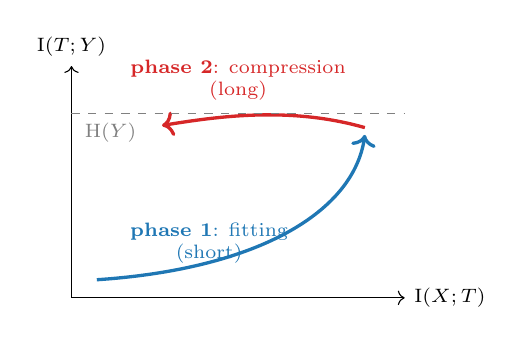
\begin{tikzpicture}[scale=0.92]
  \draw[->] (0,0)--(4.6,0) node[right, font=\scriptsize] {$\I(X;T)$};
  \draw[->] (0,0)--(0,3.2) node[above, font=\scriptsize] {$\I(T;Y)$};
  \draw[very thick, good, ->] (0.35,0.25) .. controls (2.6,0.4) and (3.9,1.2) .. (4.05,2.25);
  \draw[very thick, bad, ->]  (4.05,2.35) .. controls (3.0,2.65) and (2.0,2.5) .. (1.25,2.38);
  \node[good, font=\scriptsize, align=center] at (1.9,0.75) {\textbf{phase 1}: fitting\\(short)};
  \node[bad,  font=\scriptsize, align=center] at (2.3,3.0) {\textbf{phase 2}: compression\\(long)};
  \draw[dashed, gray] (0,2.55)--(4.6,2.55);
  \node[gray, font=\scriptsize, below right] at (0.05,2.55) {$\HH(Y)$};
\end{tikzpicture}\\[4pt]
\footnotesize
One layer's trajectory, schematically. \emph{This picture is the entire object of the
dispute} --- and we will reproduce it exactly.
\end{column}
\end{columns}
\end{frame}

\begin{frame}{Three claims (Shwartz-Ziv \& Tishby 2017)}
\begin{block}{Claim 1 --- Two phases}
Training has a \emph{fitting} phase, then a distinct \textbf{compression} phase.
\end{block}
\begin{block}{Claim 2 --- Causality}
The compression phase \textbf{explains} why deep networks generalise.
\end{block}
\begin{block}{Claim 3 --- Mechanism}
Compression is driven by the \textbf{diffusion} of stochastic gradient descent.
\end{block}
\bigskip
\begin{center}
\large Saxe et al.: \textcolor{bad}{none of the three holds in general.}\\[2pt]
\normalsize This project reproduces that argument from scratch.
\end{center}
\end{frame}

% ============================================================== the problem ==
\section{The obstruction}

\begin{frame}{The problem: deterministic networks carry infinite information}
\label{slide:problem}
For a deterministic continuous layer $h = f(X)$:
\[ \I(h;X) = \HH(h) - \underbrace{\HH(h\mid X)}_{\text{point mass}\;\Rightarrow\;-\infty} \]
\begin{center}
\begin{beamercolorbox}[sep=6pt,center,rounded=true,shadow=true]{block title}
\Large $\I(h;X) = \infty$ \quad at \emph{every} point in training
\end{beamercolorbox}
\end{center}
\medskip
A constant has no fitting phase and no compression phase.\\[4pt]
So every finite number ever plotted comes from an \textbf{added assumption}:
\begin{itemize}
  \item \textbf{binning}\; $T=\mathrm{bin}(h)$ \;$\Rightarrow$\; $\HH(T\mid X)=0$,\; $\I(T;X)=\HH(T)$
  \item \textbf{noise}\; $T=h+Z$,\; $Z\perp X$ \;$\Rightarrow$\; $\I(T;X)=\HH(T)-\HH(Z)$
\end{itemize}
\bigskip
\centering\emph{Neither is part of the network. Both are choices made by the analyst.}
\end{frame}

\begin{frame}{The two tricks --- and the price of each}
\centering\footnotesize
\begin{tabular}{@{}p{3.1cm}p{4.3cm}p{4.6cm}@{}}
\toprule
 & \textbf{Binning} & \textbf{Noise} \\
\midrule
definition & $T=\mathrm{bin}(h)$ & $T = h + Z$, \ $Z\perp X$ \\[3pt]
what it buys &
  $\HH(T\mid X)=0$, so $\I(T;X)=\HH(T)$ &
  $\I(T;X)=\HH(T)-\HH(Z)$ \\[3pt]
what you must choose &
  a \textbf{resolution} (bin edges + count) &
  a \textbf{noise level} $\smi^2$ \\[3pt]
ceiling &
  $\I \le \log_2 P$ --- set by the estimator, not the network &
  set by $\smi^2$ relative to $\|h\|$ \\[3pt]
\textcolor{bad}{the price} &
  \textcolor{bad}{move the edges and the conclusion moves} &
  \textcolor{bad}{rescale $h$ and the answer moves, though the function is unchanged} \\
\bottomrule
\end{tabular}
\medskip
\begin{beamercolorbox}[sep=4pt,center,rounded=true]{block title}
\small Both replace ``how much does the layer know about $X$?'' with\\
``\emph{how much does the layer know about $X$, \textbf{at the resolution I chose}?}''
\end{beamercolorbox}
\smallskip
{\footnotesize\centering
A third route --- $k$-nearest-neighbour --- avoids fixing $\smi^2$ by using only
$\Delta\I=\Delta\HH$. It pays for that with a different assumption: that the layer has
a density at all.\par}
\end{frame}

\begin{frame}{Two immediate casualties}
\vspace{-6pt}
\begin{center}
\begin{tikzpicture}[
  scale=0.92, every node/.style={transform shape},
  >={Stealth[length=4pt]}, font=\small,
  net/.style={draw=structure, fill=structure!12, rounded corners=2pt,
              minimum width=0.9cm, minimum height=0.55cm},
  ana/.style={draw=bad, fill=bad!8, rounded corners=2pt,
              minimum width=0.9cm, minimum height=0.55cm, text=bad},
  lab/.style={font=\scriptsize, text=neutral}]

  \node[net] (x)                    {$X$};
  \node[net, right=1.0cm of x]  (h1) {$h_1$};
  \node[net, right=1.0cm of h1] (h2) {$h_2$};
  \node[right=0.8cm of h2]      (dd) {$\cdots$};
  \node[net, right=0.8cm of dd] (hL) {$h_L$};
  \draw[->] (x)--(h1); \draw[->] (h1)--(h2); \draw[->] (h2)--(dd); \draw[->] (dd)--(hL);
  \node[lab, right=0.7cm of hL, align=left]
       {the network:\\a genuine Markov chain};

  \node[ana, below=0.85cm of h1] (t1) {$T_1$};
  \node[ana, below=0.85cm of h2] (t2) {$T_2$};
  \draw[->, bad] (h1)--(t1) node[midway, right, font=\scriptsize] {$+Z_1$};
  \draw[->, bad] (h2)--(t2) node[midway, right, font=\scriptsize] {$+Z_2$};
  \draw[->, bad, dashed] (t1)--(t2);
  \node[bad] at ($(t1)!0.5!(t2)$) {\large $\boldsymbol\times$};
  \node[lab, text=bad, right=0.55cm of t2, align=left]
       {what we \emph{plot} --- independent noise,\\added \textbf{after} training};
\end{tikzpicture}
\end{center}
\vspace{-4pt}
\begin{columns}[T]
\begin{column}{0.52\textwidth}
\begin{alertblock}{\small The DPI does not apply}
\footnotesize
$T_2$ is \textbf{not} a function of $T_1$, so no inequality relates $\I(X;T_1)$ to
$\I(X;T_2)$.\\[2pt]
\textbf{The layer ordering of the plane is not guaranteed.}
\end{alertblock}
\vspace{-5pt}
{\footnotesize our ReLU run, final $\I(X;T)$ [bits]:}\\[1pt]
\centering
{\small $8.30 \to 4.58 \to
 \textcolor{bad}{2.29 \to 3.12 \to 4.15}$}\\[1pt]
{\footnotesize \textcolor{bad}{it \emph{rises} with depth} --- impossible for $\I(X;h_l)$.}
\end{column}
\begin{column}{0.46\textwidth}
\begin{alertblock}{\small Invariance is destroyed}
\footnotesize
$\I(X;g(h))=\I(X;h)$ for invertible $g$ --- the very reason to reach for $\I$.\\[2pt]
$T=h+Z$ is \textbf{not} invariant: $Z$ enters at a \emph{fixed} scale.
\end{alertblock}
\vspace{-5pt}
\centering
{\footnotesize rescale the weights, keep the function:}\\[1pt]
{\small \SI{4.32}{bits} $\longrightarrow$ \SI{0.03}{bits}}\\[1pt]
{\footnotesize same map throughout \ (slide \ref{fig:rescale}).}
\end{column}
\end{columns}
\vspace{1pt}
\begin{center}\footnotesize
Root of both: $\I(X;T)$ compares the representation's \emph{scale} to a resolution
\textbf{we} chose.\\[1pt]
Training moves the first; the second is a constant we picked.
\end{center}
\end{frame}

% ================================================================= methods ==
\section{Method}

\begin{frame}{Four estimators, all implemented and validated}
\footnotesize
\begin{tabular}{@{}llp{4.6cm}@{}}
\toprule
\textbf{estimator} & \textbf{assumption} & \textbf{key formula} \\
\midrule
Binning & discretise $h$ & $\I(T;X)=\HH(T)=-\sum_i p_i\log p_i$ \\[3pt]
KDE bounds & $T=h+\Norm(0,\sigma^2)$ &
  $\I \le -\frac1P\sum_i\log\frac1P\sum_j e^{-\|h_i-h_j\|^2/2\sigma^2}$ \\[3pt]
Kraskov $k$-NN & $T=h+Z$, any $Z$ & $\I = \HH(T)-c$; use $k$-NN distances \\[3pt]
\textbf{Exact} (linear) & $T=\Wb X+\epsilon$ &
  $\I=\frac12\log|\Wb\Sigma_X\Wb^\top+\smi^2 I|-\frac12\log|\smi^2 I|$ \\
\bottomrule
\end{tabular}
\medskip
\begin{block}{\small Validation --- 46 checks, all passing}
\begin{itemize}\footnotesize
  \item agreement with the \textbf{original authors' code} to relative $10^{-10}$
  \item analytic cases exact: $\log_2 P$ codes, Gaussian channels, $\HH(U[0,1]^d)=0$
  \item cross-estimator: exact value lies inside the KDE bounds
  \item NumPy vs PyTorch trainers agree to $10^{-7}$ ($17\times$ faster)
\end{itemize}
\end{block}
\end{frame}

\begin{frame}{The dataset makes the measurement exact}
\begin{columns}[T]
\begin{column}{0.55\textwidth}
12 binary inputs $\Rightarrow$ all $2^{12}=4096$ patterns, \textbf{each exactly once}.
\begin{itemize}
  \item the input alphabet is finite and \emph{fully enumerated}
  \item taken uniform: $\HH(X)=\log_2 4096 = \SI{12}{bits}$ \emph{exactly}
  \item binning MI over all 4096 patterns has \textbf{no sampling error}
\end{itemize}
\medskip
Network $12$--$10$--$7$--$5$--$4$--$3$--$2$,\\
final layer two sigmoidal units.
\end{column}
\begin{column}{0.42\textwidth}
\begin{block}{So any effect we see is not noise}
$\HH(Y) = \SI{0.9992}{bits}$ --- the ceiling for $\I(T;Y)$.
\end{block}
\end{column}
\end{columns}
\end{frame}

% ============================================================== result 1 ====
\section{Claim 1: two phases}

\begin{frame}{The distinction that turns out to matter}
\vspace{-4pt}
\centering
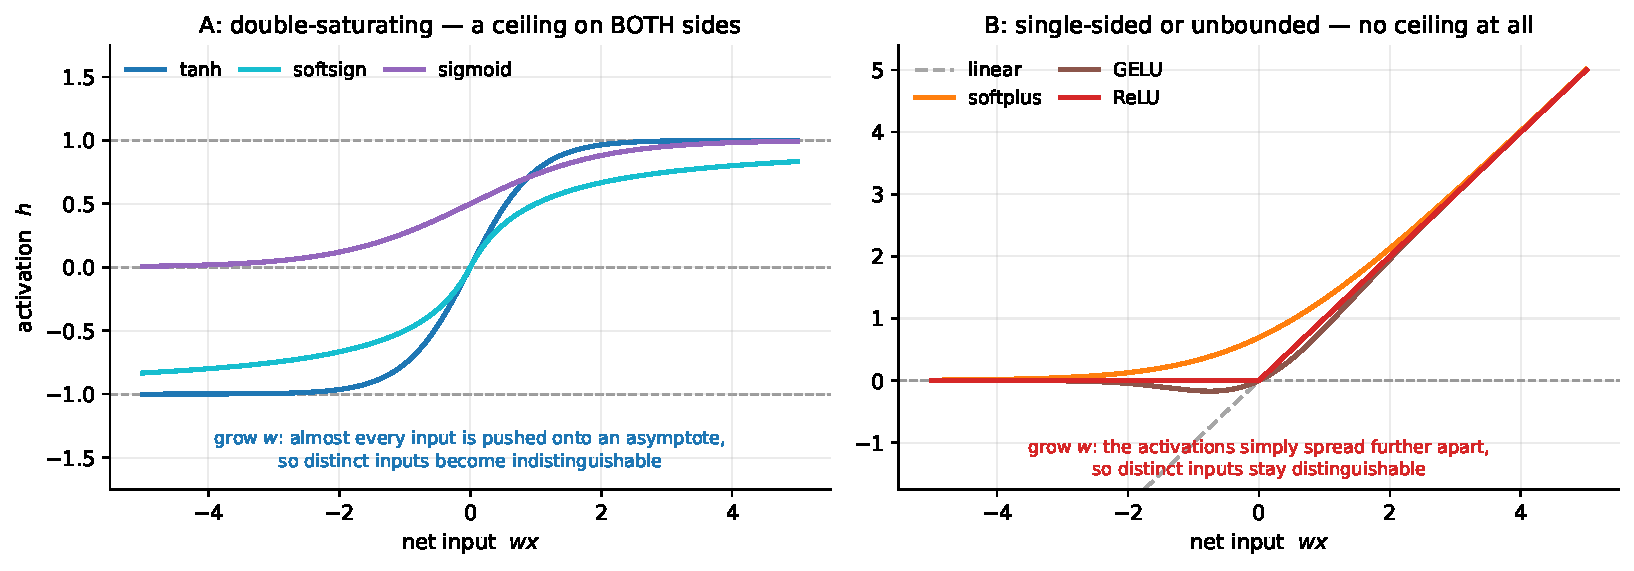
\includegraphics[width=0.80\linewidth]{fig00_activations.pdf}
\\[2pt]
\begin{columns}[T]
\begin{column}{0.50\textwidth}
\footnotesize
Not ``linear vs nonlinear'' --- whether there is a \textbf{ceiling on both sides}.
A network starts small and \emph{must grow its weights} to compute anything nonlinear;
panel A shows what that does to a bounded unit, panel B that it does nothing of the kind
to an unbounded one.\\[2pt]
\textcolor{bad}{None of this is a property of the learning algorithm.}
\end{column}
\begin{column}{0.48\textwidth}
\centering\scriptsize
\begin{tabular}{@{}lccr@{}}
\toprule
 & \textbf{bdd.\ below} & \textbf{bdd.\ above} & \textbf{compression} \\
\midrule
\texttt{tanh}     & \yes & \yes & \SI{0.69}{bits} \\
\texttt{softsign} & \yes & \yes & \SI{0.11}{bits} \\
ReLU              & \yes & \no  & \SI{0.10}{bits} \\
\texttt{softplus} & \yes & \no  & \SI{0.01}{bits} \\
\bottomrule
\end{tabular}\\[1pt]
{\scriptsize KDE, $\sigma^2 = 0.1$, 5 seeds. The ordering tracks \emph{how fast} a unit
saturates, not merely whether it is bounded.}
\end{column}
\end{columns}
\end{frame}

\begin{frame}{An exactly solvable model explains everything}
\centering
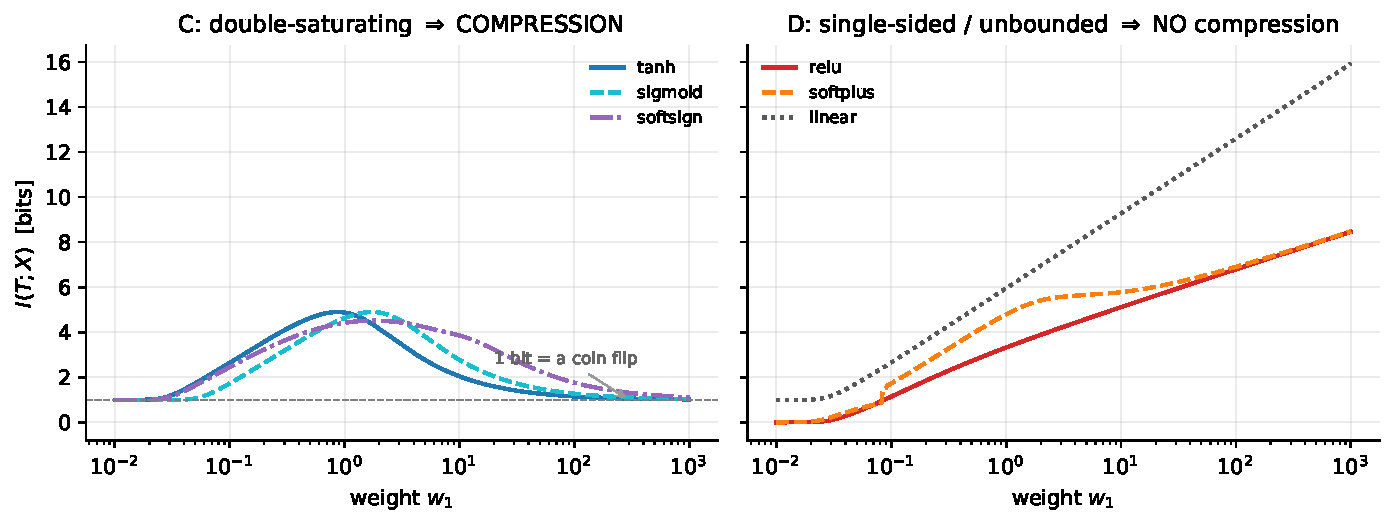
\includegraphics[width=0.92\linewidth]{fig02CD_minimal_model.pdf}
\\[4pt]
\footnotesize $X\sim\Norm(0,1)$, $h=f(w_1X)$, $T=\mathrm{bin}(h)$ --- computed \emph{exactly} from the Gaussian CDF.
\begin{itemize}\footnotesize
  \item \textbf{tanh}: rises, peaks, falls to \emph{exactly} \SI{1}{bit} (a coin flip: only the sign survives)
  \item \textbf{ReLU}: rises without bound; slope is \emph{half} the linear one (half the inputs sit in the zero bin)
\end{itemize}
\centering\emph{Networks start small and must grow their weights $\Rightarrow$ tanh traverses this curve during training.}
\end{frame}

\begin{frame}{The real network: change one word, lose the phenomenon}
\centering
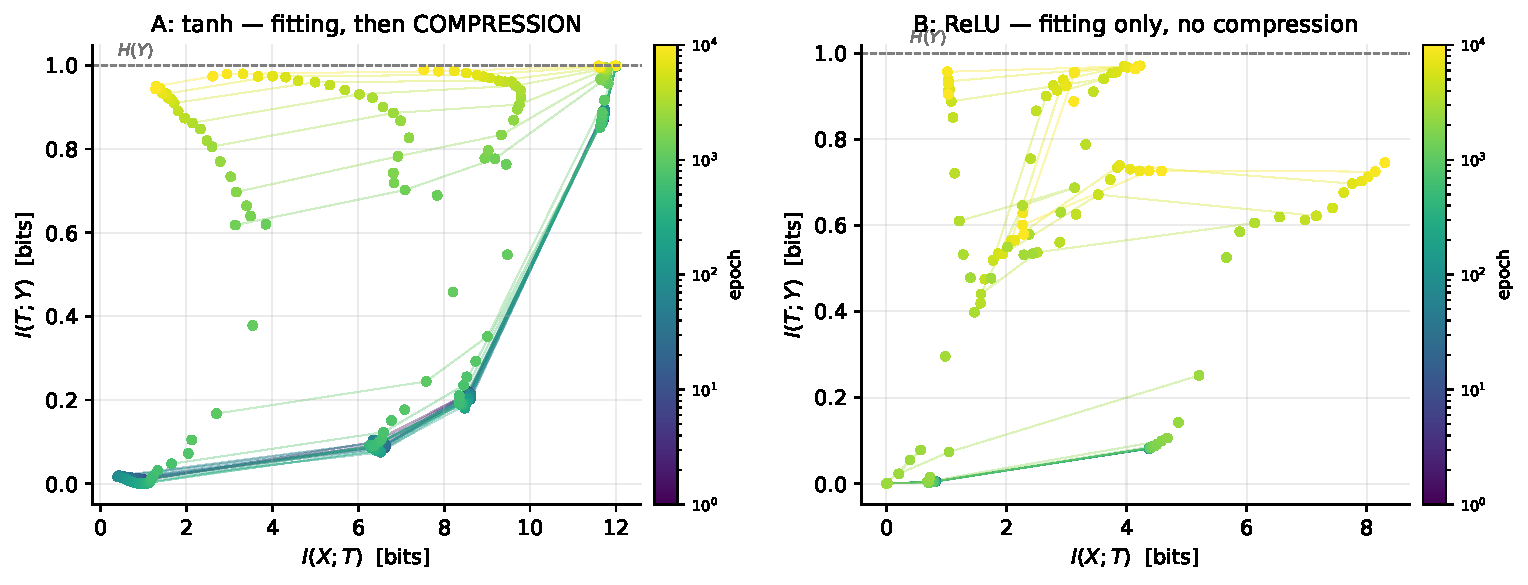
\includegraphics[width=0.98\linewidth]{fig01AB_information_plane.pdf}
\\[2pt]
\footnotesize
Identical data, identical training, identical measurement. Only \texttt{tanh}$\to$\texttt{relu}.\\
Test accuracy: \SI{96.2}{\percent} vs \SI{97.3}{\percent} --- the ReLU network is \emph{better}.\\[3pt]
The one ReLU curve that compresses is the \textbf{sigmoidal output layer}.
\end{frame}

\begin{frame}{Two of the three claims, already gone}
\begin{columns}[T]
\begin{column}{0.52\textwidth}
\begin{alertblock}{\small Claim 1 --- two phases --- \textbf{NO}}
\footnotesize
One identifier changed, \texttt{tanh}$\to$\texttt{relu}, and the compression phase is
gone: \SI{10.66}{bits} $\to$ \SI{0.47}{bits}.\\[2pt]
It is not a universal property of learning. It is a \textbf{side effect of the
nonlinearity} --- exactly what the one-neuron model predicted two slides ago.
\end{alertblock}
\vspace{-2pt}
\begin{alertblock}{\small Claim 2 --- compression causes generalisation --- \textbf{NO}}
\footnotesize
\centering
\begin{tabular}{@{}lrr@{}}
\midrule
 & compression & test acc.\ \\
\texttt{tanh} & \SI{10.66}{bits} & \SI{96.2}{\percent} \\
ReLU & \SI{0.47}{bits} & \textcolor{good}{\SI{97.3}{\percent}} \\
\midrule
\end{tabular}\\[2pt]
The network that compressed \emph{nothing} generalised \textbf{better}.
\end{alertblock}
\end{column}
\begin{column}{0.46\textwidth}
\begin{block}{\small The exception that proves the rule}
\footnotesize
One curve in the ReLU plane \emph{does} hook left --- the \textbf{output layer}. And the
output layer is not ReLU: it is \textbf{sigmoidal}, because it must produce probabilities
in $[0,1]$. Double-saturating, exactly like \texttt{tanh}.
\smallskip
\centering\scriptsize
\begin{tabular}{@{}lccccc|c@{}}
\toprule
ReLU net & L1 & L2 & L3 & L4 & L5 & \textbf{out} \\
\midrule
compression & 0.00 & 0.00 & 0.00 & 0.02 & 0.08 & \textcolor{bad}{\textbf{0.37}} \\
\bottomrule
\end{tabular}\\[3pt]
\footnotesize
The five ReLU layers compress \SI{0.10}{bits} \emph{between them}; the one sigmoid layer
compresses \SI{0.37}{} --- \SI{79}{\percent} of the network's total.
\end{block}
\end{column}
\end{columns}
\vspace{-2pt}
\begin{beamercolorbox}[sep=3pt,center,rounded=true]{block title}
\footnotesize
The mechanism predicts its own exception, and the exception is there. \ Claim 3 --- that
SGD's noise is the \emph{cause} --- is still standing; we remove that next.
\end{beamercolorbox}
\end{frame}

\begin{frame}{The mechanism, caught in the act}
\centering
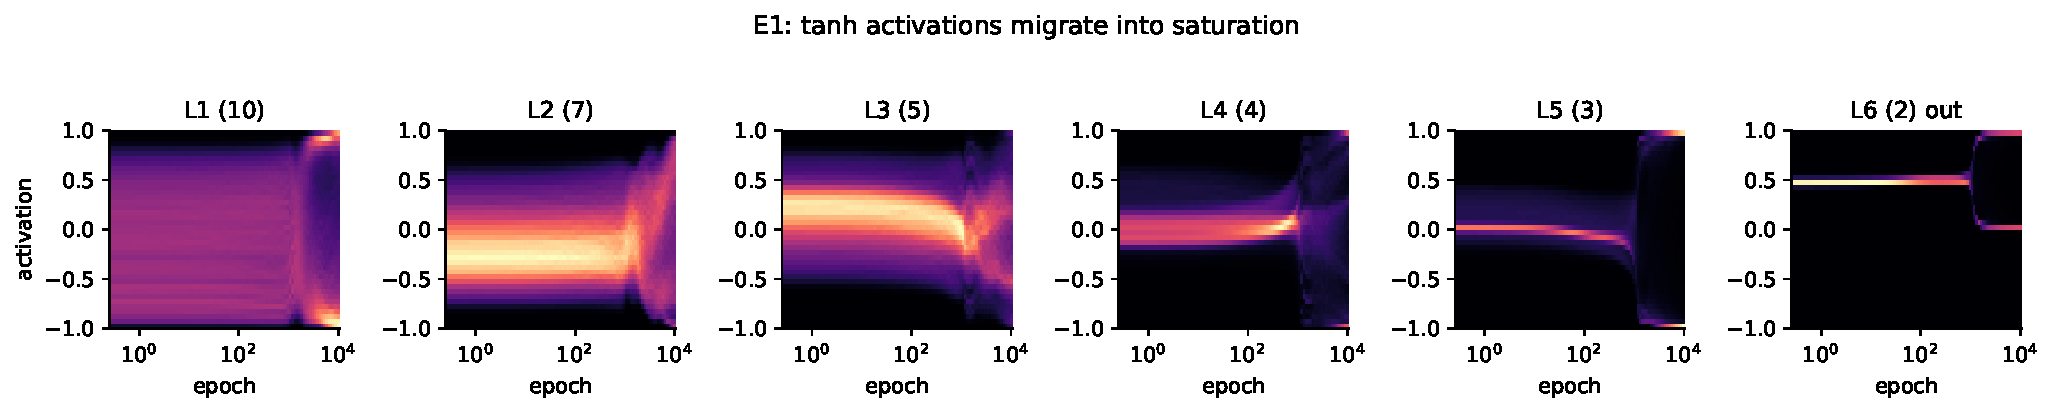
\includegraphics[width=0.98\linewidth]{figE1_tanh_activations.pdf}
\\[4pt]
\begin{columns}
\begin{column}{0.5\textwidth}\centering
\textbf{tanh}: fraction of layer-5 units saturated ($|h|>0.98$)\\[2pt]
\SI{0.0}{\percent} $\longrightarrow$ \textcolor{bad}{\SI{75.4}{\percent}}
\end{column}
\begin{column}{0.5\textwidth}\centering
\textbf{ReLU}: max activation\\[2pt]
grows without bound to \textcolor{good}{\num{56.3}}
\end{column}
\end{columns}
\end{frame}

\begin{frame}{How to read those heatmaps --- and the ReLU contrast}
\begin{columns}[T]
\begin{column}{0.46\textwidth}
\footnotesize
\textbf{One panel per layer, L1 to the output.}
\begin{itemize}\footnotesize
  \item \textbf{x}: epoch, log scale
  \item \textbf{y}: the raw activation $h$, penned into $[-1,1]$ by \texttt{tanh}
  \item \textbf{colour}: where the units actually are --- bright = most of them,
        dark = empty
\end{itemize}
\smallskip
\begin{block}{\footnotesize What the two phases look like}
\footnotesize
\textbf{Early}: one bright band at $h\approx 0$. Weights are still small, so the data
passes through the \emph{linear} middle of \texttt{tanh} undistorted.\\[3pt]
\textbf{Late}: the band \textbf{splits and migrates} to $+1$ and $-1$. The weights have
grown, and the units are saturating.
\end{block}
\smallskip
Layer 5, fraction with $|h|>0.98$: \ \SI{0.0}{\percent} $\to$ \textcolor{bad}{\SI{75.4}{\percent}}.
\end{column}
\begin{column}{0.52\textwidth}
\centering
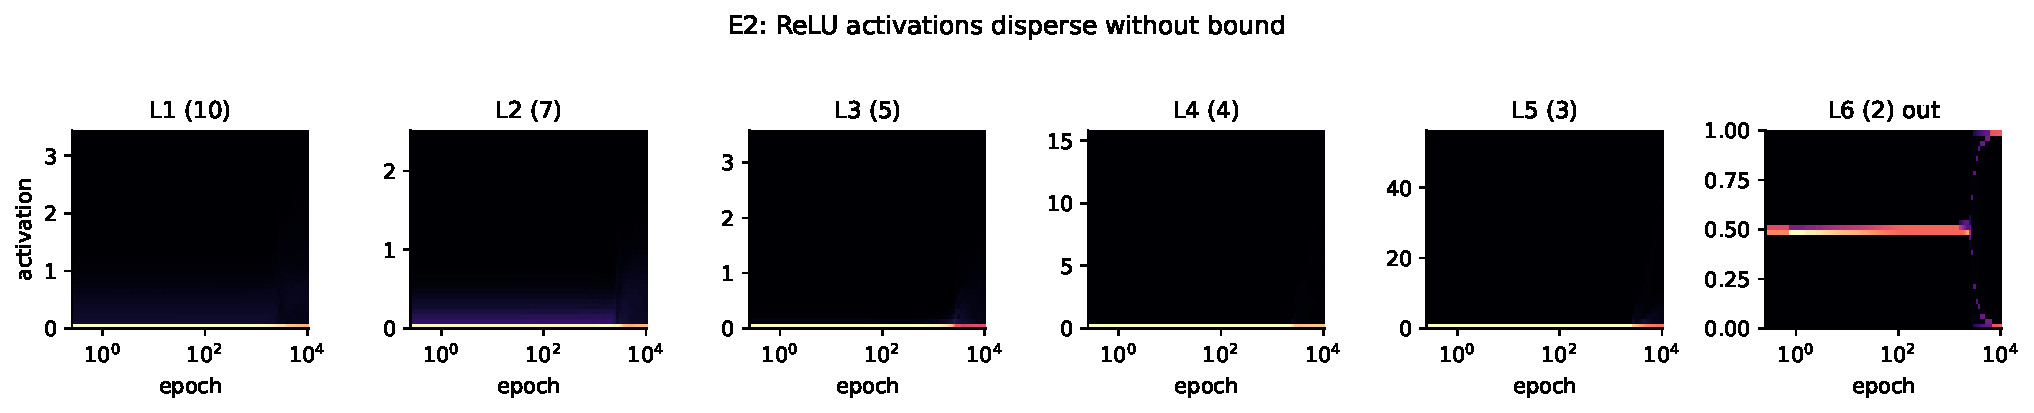
\includegraphics[width=\linewidth]{figE2_relu_activations.pdf}\\[1pt]
{\scriptsize the same plot for ReLU --- note the vertical axis}
\smallskip
\begin{alertblock}{\footnotesize Why one gives a compression phase and the other does not}
\footnotesize
Three quarters of layer 5 now sits in the outermost two bins, so the binner assigns all
of it the \emph{same two symbols}. $\HH(T)$ collapses. That mechanical pile-up against a
fixed wall is what gets read as ``a massive loss of information''.\\[3pt]
ReLU has \textbf{no wall}. As its weights grow the activations simply expand outward ---
up to \num{56.3} here --- spreading across \emph{more} bins, so the estimate never falls.
\end{alertblock}
\end{column}
\end{columns}
\end{frame}

\begin{frame}{It is the measurement, not the network}
\centering
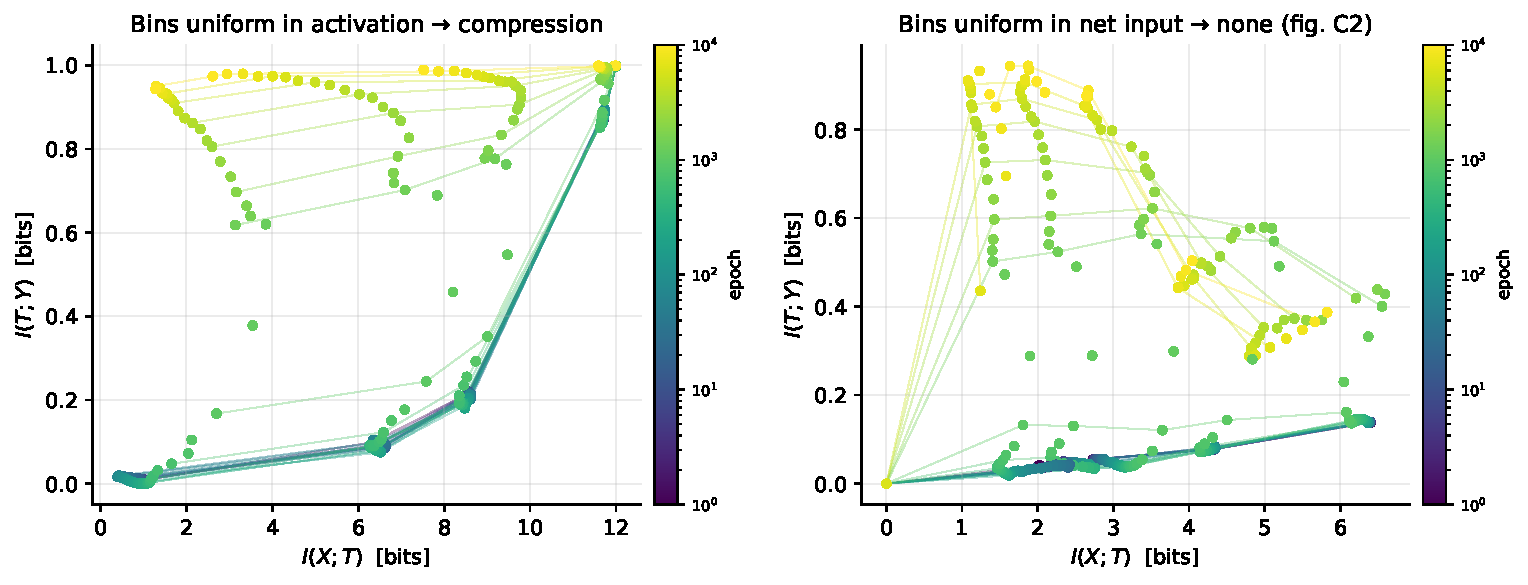
\includegraphics[width=0.84\linewidth]{figC2_binning_changes_conclusion.pdf}
\\[2pt]
Same network. Same weights. Same training run.\\
\textbf{Only the bin edges differ.}
\medskip
\begin{center}\large
layer 5 compression: \ \SI{5.59}{bits} \ $\longrightarrow$ \ \SI{0.32}{bits}
\end{center}
\footnotesize\centering
At full machine precision every input gets its own code: $\I(X;T)$ pinned at \SI{12}{bits}, no dynamics at all.
\end{frame}

% ============================================================== result 2 ====
\section{Claim 2: causality}

\begin{frame}{Take the bins away entirely: there are no dynamics at all}
\vspace{-4pt}
\centering
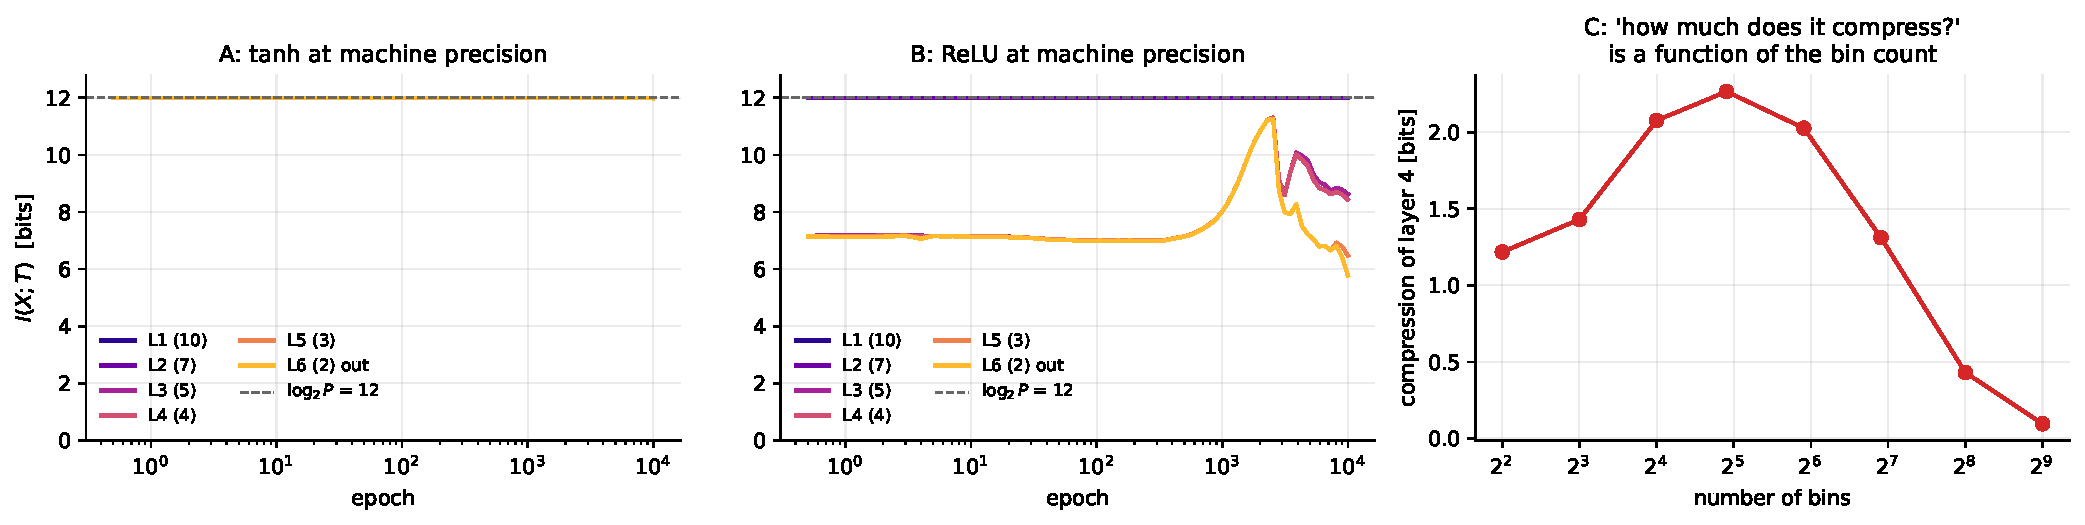
\includegraphics[width=0.80\linewidth]{fig08_resolution.pdf}
\\[2pt]
\begin{columns}[T]
\begin{column}{0.50\textwidth}
\footnotesize
Stop rounding: two activations share a symbol only if their \textbf{float32 bit patterns
are identical} --- $\sim 2^{32}$ levels, which is what the network actually computes in.
\\[2pt]
The layer is then an \textbf{injective} map --- a perfect ID tag for the input --- so
$\I(X;T)=\HH(X)=\SI{12}{bits}$ at every epoch, in every layer (panel A).
\textbf{No fitting phase, no compression phase, no dynamics: a flat line.}
\end{column}
\begin{column}{0.48\textwidth}
\footnotesize
And this is not a \emph{better estimate} of the same thing --- for a deterministic network
it is \textbf{the true value}. Slide \ref{slide:problem} said so in advance: constant for
discrete $X$, infinite for continuous $X$. Here is the constant, measured.\\[2pt]
Panel C sweeps everything in between: one layer's measured compression runs from
\SI{0.10}{} to \SI{2.27}{bits}, \emph{not even monotone} in the bin count.
\end{column}
\end{columns}
\vspace{2pt}
{\scriptsize\centering
ReLU (panel B) does not sit at 12: a unit that is off outputs \textbf{exactly} zero, so
some patterns genuinely collide --- a real atom in the distribution, and one that breaks
any estimator assuming a density.\par}
\end{frame}

\begin{frame}{Removing the estimator entirely}
\begin{columns}[T]
\begin{column}{0.52\textwidth}
\footnotesize
So far every number has depended on a choice. Take the choice away.\\[4pt]
\textbf{The model} (paper \S3) --- a linear student and a linear teacher:
\[ X\sim\Norm\big(0,\tfrac{1}{N_i}I\big),\qquad Y = W_o X + \epsilon_o \]
\[ T = \Wb X, \qquad \Wb = W_l\cdots W_1 \]
Deterministic again, so $\I(T;X)=\infty$. \emph{For the analysis only}, set
$T = \Wb X + \epsilon_{MI}$, \ $\epsilon_{MI}\sim\Norm(0,\smi^2 I)$.
\smallskip

Everything is now jointly Gaussian, hence \textbf{closed form}:
\[ \I(T;X)=\tfrac12\log\big|\Wb\Sigma_X\Wb^\top+\smi^2 I\big|
           -\tfrac12\log\big|\smi^2 I\big| \]
\[ \I(T;Y)=\HH(T)+\HH(Y)-\HH(T,Y) \]
and so is the generalisation error $E_g$ itself.\\
{\scriptsize paper eqs.\ (6), (G.1)--(G.4) and (5)}
\end{column}
\begin{column}{0.46\textwidth}
\begin{block}{\small Is a \emph{linear} network a fair test?}
\footnotesize
Yes --- it is linear in the \emph{input}, not in the learning:
\begin{itemize}\footnotesize
  \item the optimisation is still \textbf{non-convex}, the dynamics still nonlinear in
        time (Saxe, McClelland \& Ganguli 2014)
  \item it genuinely \textbf{overtrains} (Advani \& Saxe 2017)
  \item a linear map can correlate neurons and project directions out --- the two
        mechanisms usually offered for compression
\end{itemize}
\end{block}
\vspace{-3pt}
\begin{alertblock}{\small What is gone}
\footnotesize
No bins, no bandwidth, no neighbours. $E_g$ is the \emph{exact expected} error, not a
test-set estimate. One assumption remains, $\smi^2$, and it is written down.
\end{alertblock}
\vspace{-1pt}
\centering\footnotesize
We look for one thing: \textcolor{bad}{\textbf{any leftward motion at all.}}
\end{column}
\end{columns}
\end{frame}

\begin{frame}{No compression --- at any depth, under any optimiser}
\begin{columns}[T]
\begin{column}{0.42\textwidth}
\footnotesize
\textbf{Top row} (paper fig.\ 3) --- full-batch GD, a network that \emph{generalises}.\\[2pt]
\textbf{Bottom row} (paper fig.\ 4) --- SGD, $b=5$, at $P=N_i$: the interpolation peak,
where linear networks overtrain worst.\\[4pt]
Left panels are the learning curves; right panels are the \textbf{exact} information plane.
\smallskip
\centering
\begin{tabular}{@{}lrr@{}}
\toprule
 & compression & final $E_g$ \\
\midrule
generalises & \SI{0.00000}{bits} & 1.61 \\
overtrains  & \SI{0.00000}{bits} & \textcolor{bad}{20.30} \\
\bottomrule
\end{tabular}\\[2pt]
{\scriptsize irreducible floor $\sigma_o^2 = 1.00$}
\smallskip

\raggedright
Both planes run monotonically \textbf{right}. Zero leftward motion --- any layer, up to six
hidden layers, SGD or BGD, 500 or \num{20000} epochs.
\end{column}
\begin{column}{0.56\textwidth}
\centering
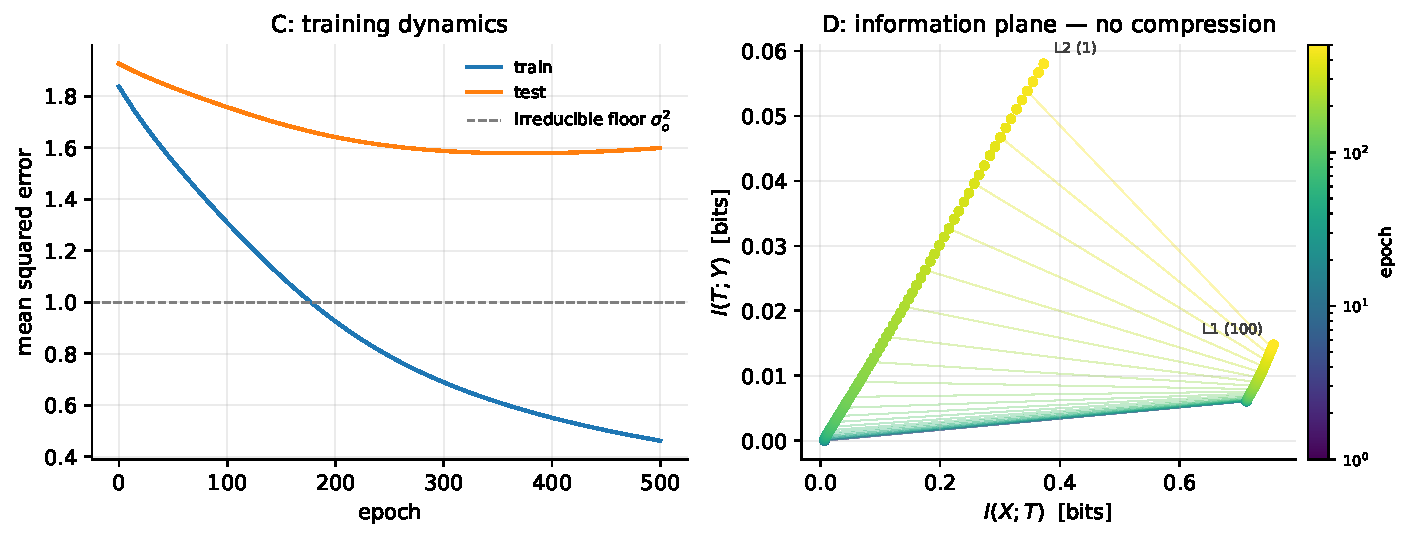
\includegraphics[width=\linewidth]{fig03CD_linear_bgd.pdf}\\[2pt]
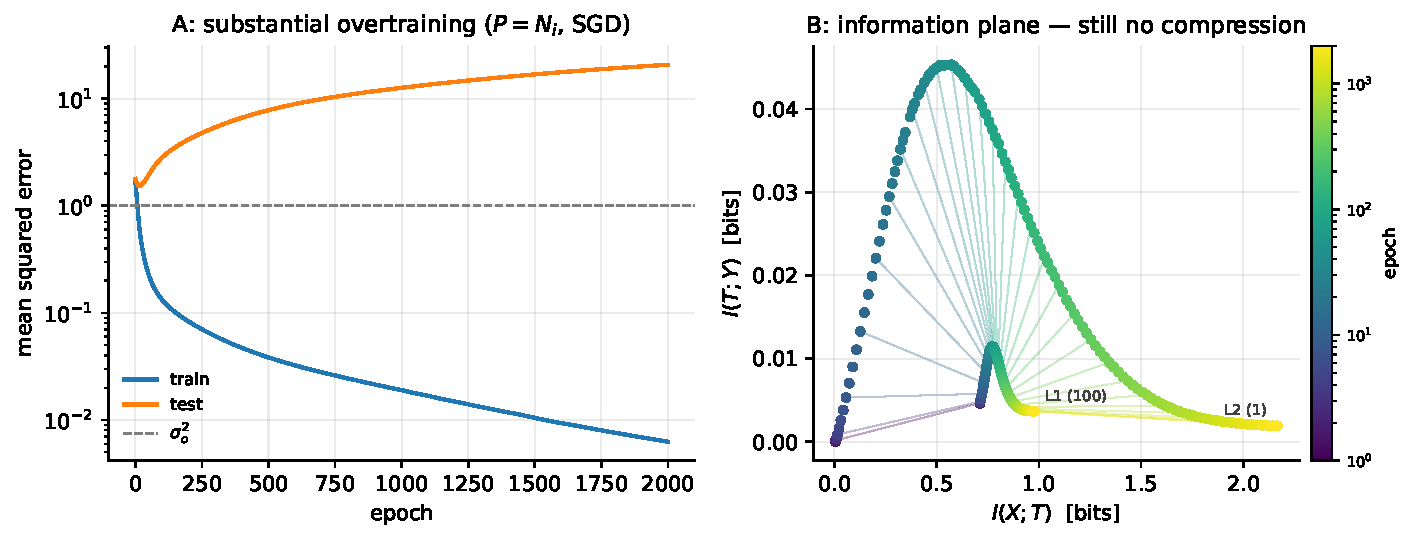
\includegraphics[width=\linewidth]{fig04AB_linear_overfit.pdf}
\end{column}
\end{columns}
\vspace{-2pt}
{\scriptsize
Panel \textbf{B} \emph{does} show the overtraining --- on the \textbf{y}-axis: $\I(T;Y)$
rises, then falls as the network memorises. The $x$-axis never turns: the plane sees the
failure, but the \emph{compression} coordinate is not what registers it.\par}
\end{frame}

\begin{frame}{The dissociation}
\centering
\small
\begin{tabular}{lrcrc}
\toprule
\textbf{network} & \textbf{compression} & \textbf{compresses?}
                 & \textbf{gap} & \textbf{generalises?} \\
\midrule
\texttt{tanh}, \SI{80}{\percent} data & \SI{10.66}{bits} & \yes & 0.019 & \yes \\
ReLU, \SI{80}{\percent} data          & \SI{0.47}{bits}  & \no  & 0.014 & \yes \\
\texttt{tanh}, \SI{30}{\percent} data & \SI{7.99}{bits}  & \yes & 0.063 & \no  \\
ReLU, \SI{30}{\percent} data          & \SI{0.62}{bits}  & \no  & 0.055 & \no  \\
\midrule
linear, BGD                           & \SI{0.00}{bits}  & \no  & $1.6\times$ & \yes \\
linear, SGD $b{=}5$                   & \SI{0.00}{bits}  & \no  & $20.3\times$ & \no \\
\bottomrule
\end{tabular}
\bigskip
\begin{center}
\Large All four combinations occur.\\[3pt]
\normalsize Neither implies the other.
\end{center}
\end{frame}

\begin{frame}{Same function, different ``information''}
\label{fig:rescale}
\begin{columns}[T]
\begin{column}{0.5\textwidth}
Take $\hat{y}=w_2w_1x$ and rescale
\[ \tilde{w}_1 = w_1/c,\qquad \tilde{w}_2 = c\,w_2. \]
Every member computes the \textbf{same map} $\Rightarrow$ generalises identically.\\[6pt]
But
\[ \I(T;X)=\tfrac12\log\frac{w_1^2/c^2+\smi^2}{\smi^2} \]
depends on $c$.
\medskip
\begin{center}
\SI{4.32}{bits} $\longrightarrow$ \SI{0.03}{bits}\\
\footnotesize for an \emph{unchanged} input--output map
\end{center}
\end{column}
\begin{column}{0.48\textwidth}
\centering
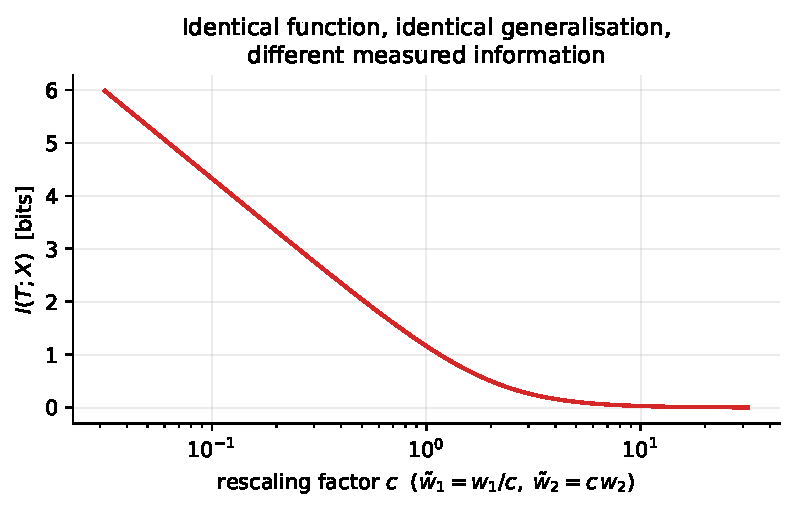
\includegraphics[width=\linewidth]{figC5_rescaling.pdf}
\end{column}
\end{columns}
\end{frame}

% ============================================================== result 3 ====
\section{Claim 3: SGD diffusion}

\begin{frame}{Remove the randomness entirely}
Full-batch gradient descent: no sampling noise, no diffusion, deterministic updates.
\bigskip
\centering
\small
\begin{tabular}{lrrrrrrr}
\toprule
& L1 & L2 & L3 & L4 & L5 & L6 & \textbf{total} \\
\midrule
\texttt{tanh}, SGD & 0.00 & 0.02 & 0.23 & 2.27 & 5.59 & 2.56 & \textbf{10.66} \\
\texttt{tanh}, \textbf{BGD} & 0.01 & 1.34 & 3.30 & 3.86 & 6.52 & 2.84 & \textcolor{bad}{\textbf{17.87}} \\
ReLU, SGD & 0.00 & 0.00 & 0.00 & 0.02 & 0.08 & 0.37 & 0.47 \\
ReLU, \textbf{BGD} & 0.00 & 0.00 & 0.00 & 0.03 & 0.11 & 0.00 & 0.13 \\
\bottomrule
\end{tabular}
\bigskip
\begin{center}
\Large Deterministic training compresses \emph{more}.\\[3pt]
\normalsize The prediction fails --- in the wrong direction.
\end{center}
\end{frame}

% ============================================================== conclusion ==
\section{Conclusions}

\begin{frame}{Results, and what they mean}
\centering\footnotesize
\begin{tabular}{@{}L{3.4cm}L{3.7cm}L{5.1cm}@{}}
\toprule
\textbf{the claim} & \textbf{the test} & \textbf{the result} \\
\midrule
\addlinespace[2pt]
\textbf{1.} Training has two phases, the second being compression &
  change \texttt{tanh}$\to$\texttt{relu}, and nothing else &
  \SI{10.66}{} $\to$ \SI{0.47}{bits}, and the ReLU network is \emph{more} accurate
  (\SI{97.3}{} vs \SI{96.2}{\percent}) \ \no \\
\addlinespace[6pt]
\textbf{2.} Compression causes generalisation &
  exact mutual information in deep linear networks &
  \SI{0.00000}{bits} in both, while $E_g$ differs by $13\times$ (1.61 vs 20.30) \ \no \\
\addlinespace[6pt]
\textbf{3.} SGD's diffusion is the cause &
  deterministic full-batch gradient descent &
  \SI{17.87}{bits} vs \SI{10.66}{} --- \emph{more} compression with no noise at all \ \no \\
\addlinespace[2pt]
\bottomrule
\end{tabular}
\medskip
\begin{columns}[T]
\begin{column}{0.52\textwidth}
\begin{alertblock}{\small The deeper point}
\footnotesize
For a deterministic network $\I(X;T)$ is $\infty$ (continuous $X$) or a \emph{constant}
(discrete $X$) --- measured at machine precision, a flat line at \SI{12}{bits}.\\[3pt]
Every finite number ever plotted is therefore a joint property of the network \textbf{and}
an assumption the analyst added.
\end{alertblock}
\end{column}
\begin{column}{0.46\textwidth}
\begin{block}{\small What survives}
\footnotesize
The saturation is \textbf{real}: \texttt{tanh} units genuinely do pile up against
$\pm 1$ (\SI{0}{} $\to$ \SI{75.4}{\percent}).\\[3pt]
What fails is the step from that to \emph{``the layer discarded ten bits about the
input''}.
\end{block}
\end{column}
\end{columns}
\end{frame}

\begin{frame}{One slide to take away}
\begin{beamercolorbox}[sep=8pt,center,rounded=true,shadow=true]{block title}
\large
Hold the network fixed. Change only how you \emph{measure} it.\\[4pt]
\normalsize
bin edges: \ layer 5 compresses \SI{5.59}{bits} \ $\longrightarrow$ \ \SI{0.32}{bits}\\
bin count: \ the same layer, \SI{0.10}{} \ $\longrightarrow$ \ \SI{2.27}{bits}, non-monotone\\
full precision: \ a flat line at \SI{12}{bits}, no dynamics at all\\
rescale the weights, same function: \ \SI{4.32}{} \ $\longrightarrow$ \ \SI{0.03}{bits}
\end{beamercolorbox}
\bigskip
\begin{center}
\large
The information plane is a picture of a network \emph{and} a ruler.\\[3pt]
\normalsize
Before attributing a trajectory to learning, check it is not a property of the ruler.
\end{center}
\end{frame}

\begin{frame}[plain]
\begin{center}
\Huge Thank you\\[10pt]
\normalsize Questions?
\end{center}
\end{frame}

\end{document}
